\documentclass[a4paper,12pt]{jarticle}
\usepackage[dvipdfmx]{graphicx}
\usepackage{amsmath,amssymb}
\usepackage{subfigure}
\usepackage{comment}
\usepackage{array}
\usepackage{setspace} % setspaceパッケージのインクルード
\usepackage{ascmac}
%\usepackage{fancybx}

\setlength{\hoffset}{0cm}
\setlength{\oddsidemargin}{-3mm}
\setlength{\evensidemargin}{-3cm}
\setlength{\marginparsep}{0cm}
\setlength{\marginparwidth}{0cm}
\setlength{\textheight}{24.7cm}
\setlength{\textwidth}{17cm}
\setlength{\topmargin}{-45pt}


\renewcommand{\baselinestretch}{1.6}
\renewcommand{\floatpagefraction}{1}
\renewcommand{\topfraction}{1}
\renewcommand{\bottomfraction}{1}
\renewcommand{\textfraction}{0}
\renewcommand{\labelenumi}{(\roman{enumi})}
%\renewcommand{\figurename}{Fig.} %図をFig.にする
\renewcommand{\baselinestretch}{1}

%図のキャプションからコロン:を消す
\makeatletter
\long\def\@makecaption#1#2{% #1=図表番号、#2=キャプション本文
\sbox\@tempboxa{#1. #2}
\ifdim \wd\@tempboxa >\hsize
#1 #2\par 
\else
\hb@xt@\hsize{\hfil\box\@tempboxa\hfil}
\fi}
\makeatother

\begin{document}
%
\title{\vspace{-30mm} \fbox{\large{計算数学特論~レポート課題2~~~機械知能工学専攻~~16344217~~津上~祐典}}}
\date{}
%
\maketitle
%
\vspace{-30mm}
%\parindent = 0pt %すべての段落で字下げをしない
%
%%%%%%%%%%%%%%%%%%%%%%%%%%%%%%%%%%%%%%%%%%%%%%%%%%%%%%%%%
\setlength{\abovedisplayskip}{0pt} % 数式上部のマージン
\setlength{\belowdisplayskip}{0pt} % 数式下部のマージン
%\setstretch{1.3} % ページ全体の行間を設定
%%%%%%%%%%%%%%%%%%%%%%%%%%%%%%%%%%%%%%%%%%%%%%%%%%%%%%%%%%

%%%%%%%%%%%%%%%%%%%%%%%%%%%%%%
\section*{課題1}
%%%%%%%%%%%%%%%%%%%%%%%%%%%%%%
\vspace{-4mm}
$a=7$は$p=23$の原始元であるので空欄を埋めると以下のようになる.
%
\begin{figure}[hbp]
 \begin{center}
  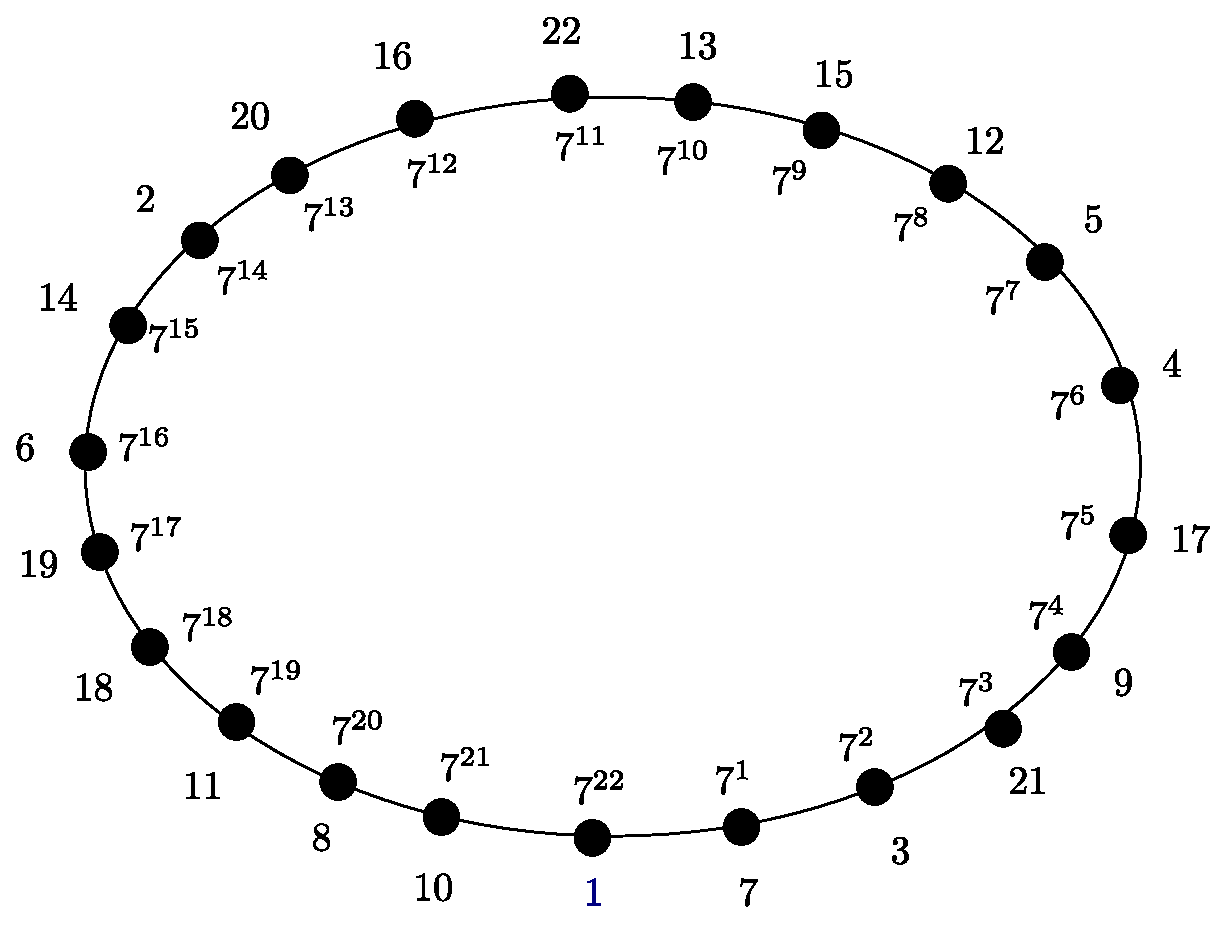
\includegraphics[width=100mm]{fig/elga.eps}
 \end{center}
 %\caption{}
 \label{fig:elga}
\end{figure}
%
\\秘密鍵を$x=20$とすると公開鍵は
%
\begin{align}
 p&=23 \\
 g&=7 \\
 y&=g^x (\mathrm{mod}~23)=7^{20}=(7^2)^{10}=3^{10}=(3^3)^3\cdot3=4^3\cdot3=8
\end{align}
%
となる.次に乱数$k=9$とし$M=5$を送信する.これ暗号化すると,
%
\begin{align}
 C_1&=g^k (\mathrm{mod}~23)=7^9=15\\
 C_2&=M \cdot y^k (\mathrm{mod}~23)=5\cdot8^9=5\cdot8 \cdot(8^2)^4 =17\cdot18^4=17\cdot18^2\cdot18^2 =17\cdot2\cdot2=22 
\end{align}
%
となる.また,復号化すると,
%
\begin{align}
 M'&=C_2\cdot \left\{ (C_1)^x \right\}^{-1} (\mathrm{mod}~23)=22\cdot \left\{15^{20}\right\}^{-1} =22\cdot 15^2=22\cdot18=5
\end{align}
%
となり$M$と一致する.
\vspace{-5mm}
%%%%%%%%%%%%%%%%%%%%%%%%%%%%%%
\section*{課題2}
%%%%%%%%%%%%%%%%%%%%%%%%%%%%%%
\vspace{-3mm}
%%%%%%%%%%%%%%%%%%%%%%%%%%%%%%%%%%%%%
\subsection*{(1)~$p=23$の原始元を全部求めよ.}
%%%%%%%%%%%%%%%%%%%%%%%%%%%%%%%%%%%%%
\vspace{-3mm}
$p=23$の約数は$1,2,11,22$である,またフェルマーの小定理より
$a^{23-1}=a^{22}=1$であるから,
%
\begin{align*}
 2^1&=2~,~2^2=4~,~2^{11}=2\cdot2^5\cdot2^5=2\cdot9\cdot9=1 \nonumber\\
 3^1&=3~,~3^2=9~,~3^{11}=(3^3)^2\cdot3^2=4^3\cdot9=18\cdot9=1 \nonumber\\
 4^1&=4~,~4^2=16~,~4^{11}=(4^3)^3\cdot4^2=18^3\cdot16=18\cdot18\cdot18\cdot16=2\cdot2=1\nonumber\\
 5^1&=5~,~5^2=25=2~,~5^{11}=(5^2)^5\cdot5=2^5\cdot5=9\cdot5=22\nonumber\\
 6^1&=6~,~6^2=36=13~,~6^{11}=(6^2)^5\cdot6=13^5\cdot6=13^2\cdot13^2\cdot13\cdot6=8\cdot8\cdot9=18\cdot9=1\nonumber\\
 7^1&=7~,~7^2=49=3~,~7^{11}=(7^2)^5\cdot7=3^5\cdot7=3^3\cdot3^2\cdot7=4\cdot9\cdot7=13\cdot7=22\nonumber\\
 8^1&=8~,~8^2=64=18~,~8^{11}=(8^2)^5\cdot8=18^5\cdot8=18^2\cdot18^2\cdot18\cdot8=2\cdot2\cdot6=1\nonumber\\
 9^1&=9~,~9^2=81=12~,~9^{11}=(9^2)^5\cdot9=12^5\cdot9=12^2\cdot12^2\cdot12\cdot9=6\cdot6\cdot16=6\cdot4=1\nonumber\\
 10^1&=10~,~10^2=100=8~,~10^{11}=(10^2)^5\cdot10=8^5\cdot10=8^2\cdot8^2\cdot8\cdot10=18\cdot18\cdot11=22\nonumber\\
 11^1&=11~,~11^2=121=6~,~11^{11}=(11^2)^5\cdot11=6^5\cdot11=6^2\cdot6^2\cdot6\cdot11=13\cdot13\cdot20=13\cdot7=22\nonumber
\end{align*}
%
  \begin{align*}
 12^1&=12~,~12^2=144=6~,~12^{11}=(12^2)^5\cdot12=6^5\cdot12=6^2\cdot6^2\cdot6\cdot12=13\cdot13\cdot3=13\cdot16=1\nonumber\\
 13^1&=13~,~13^2=169=8~,~13^{11}=(13^2)^5\cdot13=8^5\cdot11=8^2\cdot8^2\cdot8\cdot13=18\cdot18\cdot12=2\cdot12=1\nonumber\\
 14^1&=14~,~14^2=196=12~,~14^{11}=(14^2)^5\cdot14=12^5\cdot11=12^2\cdot12^2\cdot12\cdot14=6\cdot6\cdot7=13\cdot7=22\nonumber\\
 15^1&=15~,~15^2=225=18~,~15^{11}=(15^2)^5\cdot15=18^5\cdot15=18^2\cdot18^2\cdot18\cdot15=2\cdot2\cdot17=22\nonumber\\
 16^1&=16~,~16^2=256=3~,~16^{11}=(16^2)^5\cdot16=3^5\cdot16=3^3\cdot3^2\cdot16=4\cdot6=1\nonumber\\
 17^1&=17~,~17^2=289=13~,~17^{11}=(17^2)^5\cdot17=13^5\cdot17=13^2\cdot13^2\cdot13\cdot17=8\cdot8\cdot14=18\cdot14=22\nonumber\\
 18^1&=18~,~18^2=324=2~,~18^{11}=(18^2)^5\cdot18=2^5\cdot18=2^5\cdot18=9\cdot18=1\nonumber\\
 19^1&=19~,~19^2=361=6~,~19^{11}=(19^2)^5\cdot19=16^5\cdot19=16^2\cdot16^2\cdot16\cdot19=3\cdot3\cdot5=22\nonumber\\
 20^1&=20~,~20^2=400=9~,~20^{11}=(20^2)^5\cdot20=9^5\cdot20=9^2\cdot9^2\cdot9\cdot20=12\cdot12\cdot19=6\cdot19=22\nonumber\\
 21^1&=21~,~21^2=441=4~,~21^{11}=(21^2)^5\cdot21=4^5\cdot21=4^3\cdot4^2\cdot21=18\cdot4\cdot15=18\cdot14=22\nonumber\\
 22^1&=11~,~22^2=484=1\nonumber
  \end{align*}
%
より,$p=23$の原始元は$5,7,10,11,14,15,17,19,20,21$である.
\vspace{-6mm}
%%%%%%%%%%%%%%%%%%%%%%%%%%%%%%%%%%%%%%%
\subsection*{(2)~原始元$\alpha$,乱数$a,b$を与えて共有鍵を持てることを確認せよ.}
%%%%%%%%%%%%%%%%%%%%%%%%%%%%%%%%%%%%%%%
\vspace{-3mm}
$\alpha=7$とする.
\vspace{-6mm}
%%%%%%%%%%%%%%%%%%%%%%%%%%%%%%%%
\subsubsection*{1.~$a=6,b=9$のとき}
%%%%%%%%%%%%%%%%%%%%%%%%%%%%%%%%
\vspace{-4mm}
$\alpha^a,\alpha^b$を求めると課題1よりそれぞれ,
%
\begin{align}
 \alpha^a&=7^6(\mathrm{mod}~23)=4 \\
 \alpha^b&=7^9(\mathrm{mod}~23)=15
\end{align}
%
となり,$\alpha^{ab}$はそれぞれ,
%
\begin{align}
 \alpha^{ab}&=(\alpha^b)^a=15^6(\mathrm{mod}~23)=(15^2)^3=18^3=18^2\cdot18=2\cdot18=13\\
 \alpha^{ab}&=(\alpha^a)^b=4^9(\mathrm{mod}~23)=(4^3)^3=18^3=13
\end{align}
%
となり一致する.
\vspace{-6mm}
%%%%%%%%%%%%%%%%%%%%%%%%%%%%%%%%
\subsubsection*{2.~$a=14,b=16$のとき}
%%%%%%%%%%%%%%%%%%%%%%%%%%%%%%%%
\vspace{-4mm}
$\alpha^a,\alpha^b$を求めると課題1よりそれぞれ,
%
\begin{align}
 \alpha^a&=7^{14}(\mathrm{mod}~23)=2 \\
 \alpha^b&=7^{16}(\mathrm{mod}~23)=6
\end{align}
%
となり,$\alpha^{ab}$はそれぞれ,
%
\begin{align}
 \alpha^{ab}&=(\alpha^b)^a=6^{14}(\mathrm{mod}~23)=(6^2)^7=13^7=8\cdot8\cdot8\cdot13=18\cdot12=9\\
 \alpha^{ab}&=(\alpha^a)^b=2^{16}(\mathrm{mod}~23)=2^5\cdot2^5\cdot2^6=9\cdot9\cdot18=12\cdot18=9
\end{align}
%
となり一致する.
\vspace{-6mm}
%%%%%%%%%%%%%%%%%%%%%%%%%%%%%%%%
\subsubsection*{3.~$a=20,b=7$のとき}
%%%%%%%%%%%%%%%%%%%%%%%%%%%%%%%%
\vspace{-4mm}
$\alpha^a,\alpha^b$を求めると課題1よりそれぞれ,
%
\begin{align}
 \alpha^a&=7^{20}(\mathrm{mod}~23)=8 \\
 \alpha^b&=7^{7}(\mathrm{mod}~23)=5
\end{align}
%
となり,$\alpha^{ab}$はそれぞれ,
%
\begin{align}
 \alpha^{ab}&=(\alpha^b)^a=5^{20}(\mathrm{mod}~23)=(5^2)^{10}=2^{10}=2^5\cdot2^5=9\cdot9=12\\
 \alpha^{ab}&=(\alpha^a)^b=8^7(\mathrm{mod}~23)=(8^2)^3\cdot8=18^3\cdot8=18^2\cdot(18\cdot8)=2\cdot6=12
\end{align}
%
となり一致する.
\end{document}
